\documentclass{ecam}

\usepackage[utf8]{inputenc}
\usepackage[french]{babel}
\usepackage[T1]{fontenc}
\usepackage{lmodern}
\usepackage{graphicx}

% Change font to sans-serif
\renewcommand\familydefault{\sfdefault}

% Chapter title customization
\usepackage{titlesec, blindtext, color}
\definecolor{gray75}{gray}{0.75}
\newcommand{\hsp}{\hspace{20pt}}
\titleformat{\chapter}[hang]{\Huge\bfseries}{\thechapter\hsp\textcolor{gray75}{|}\hsp}{0pt}{\Huge\bfseries}
\titlespacing*{\chapter}{0pt}{30pt}{15pt}

\usepackage{etoolbox}
\makeatletter
\patchcmd{\chapter}{\if@openright\cleardoublepage\else\clearpage\fi}{}{}{}
\makeatother

% table padding
\renewcommand{\arraystretch}{1.5}

% Appendix chapters
\usepackage{appendix}

% Paragraph spacing
\setlength{\parindent}{0em}
\setlength{\parskip}{1em}

% Lists
\usepackage[shortlabels]{enumitem}

% Allows rendering images 'here' with the H option
\usepackage{float}

% Code syntax highlighting
\usepackage{minted}



\begin{document}
% Title
\title{Projet Génie logiciel \\\vspace{10pt}\fontsize{30pt}{60pt}\selectfont{KitBox}}
\author{William De Decker \& Mathieu David \& Saïkou Barry Ahmadou \linebreak \& Jonathan Petit \& Momo Guy Donatien}
\maketitle

\chapter{Introduction}
Les diagrammes suivants sont les représentations de l'application KitBox fesant l'objet du projet Génie Logiciel. Le diagramme de classe est une représentation de l'intéraction entre les différentes classes du code à venir tandis que les diagrammes de séquence et d'activité offre une vue du déroulement de la réalisation d'une armoire.
Le diagramme d'entité-relation quant à lui représente les tables dans la base donnée et les relations qu'elles ont entre elles.
Enfin, vous trouverez à la fin de ce document un diagramme des cas d'utilisations montrant les actions que les différents intervenants pourrons faire au travers notre applications.


\pagebreak
\chapter{Diagrammes}

\section{Diagramme de classe}

\begin{center}

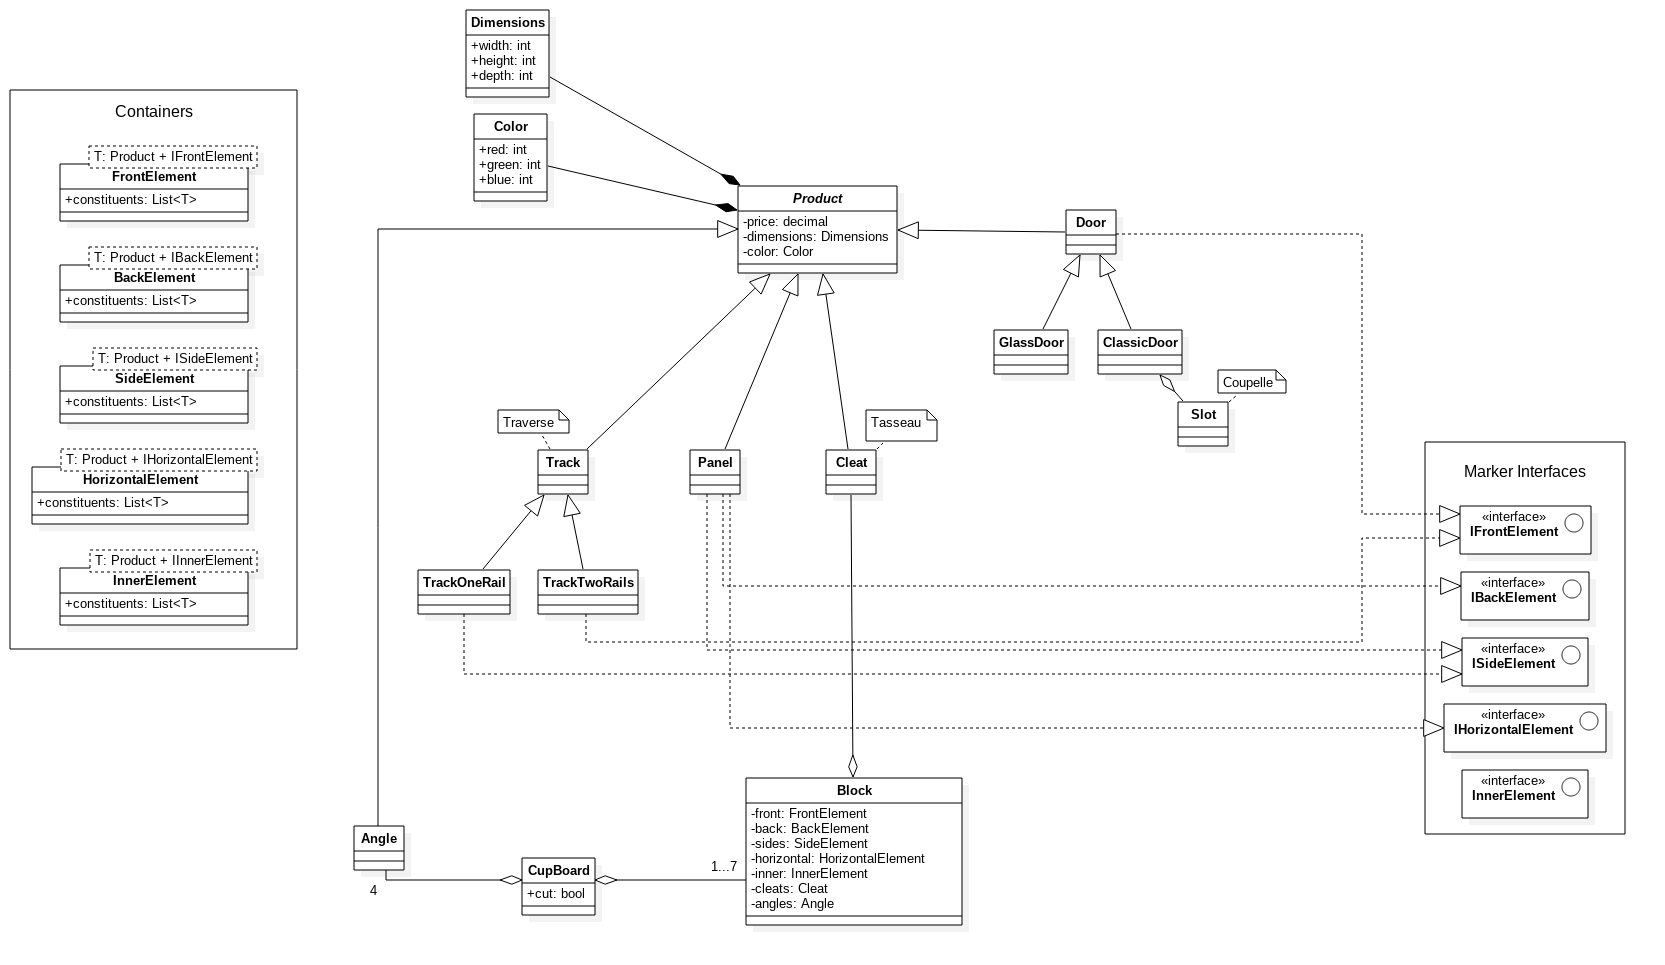
\includegraphics[angle=270,scale=0.3]{../images/class-diagram.png}
\end{center}

\section{Diagramme de Séquence}

\section{Diagramme d'activité}

\begin{center}
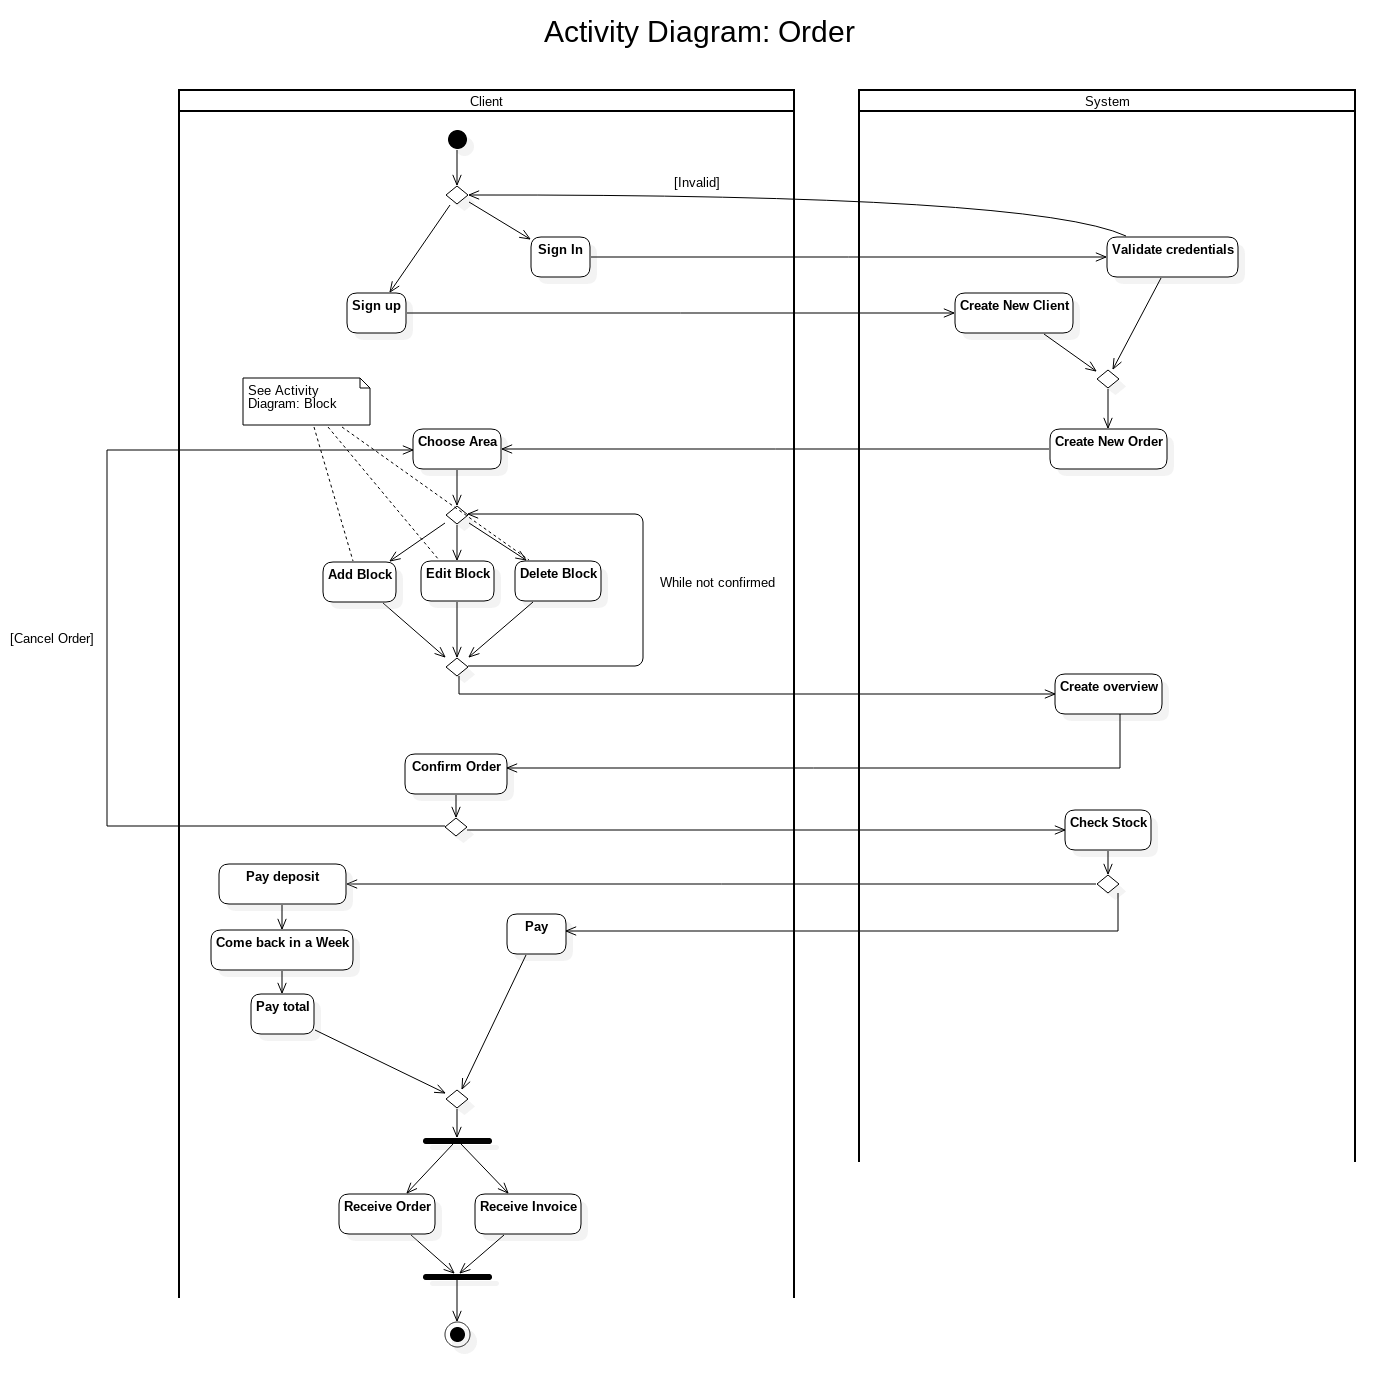
\includegraphics[angle=0,scale=0.3]{../images/activity-diagram.png}
\end{center}

\section{Diagramme d'entité-relation}

\begin{center}

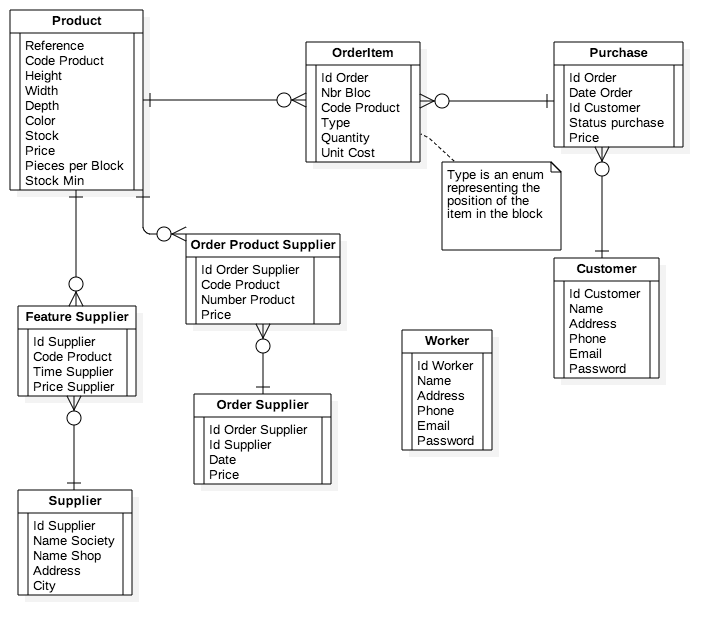
\includegraphics[angle=0,scale=0.3]{../images/ERDDiagram.png}

\end{center}

\section{Diagramme des cas d'utilisation}
\begin{center}

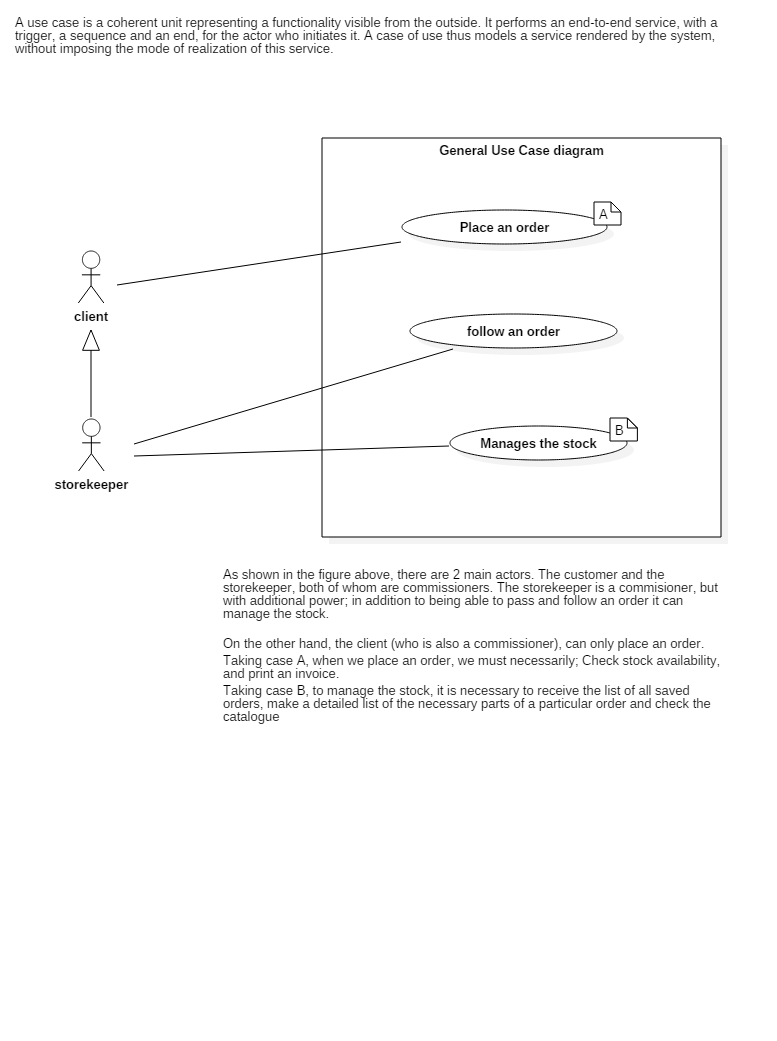
\includegraphics[angle=0,scale=0.3]{../images/use-case-diagram.png}
\end{center}

\end{document}
